\documentclass[11pt]{article}

\newcommand{\pset}{
    2
}
\newcommand{\subtitle}{
    Language Acceptance; 
    Finite and Infinite Automata;
    Finitely Recognizable Languages
}
\newcommand{\duedate}{
    Friday, September 12
}

% Page Setup
\usepackage{geometry}
\geometry{
    a4paper,
    margin={2.5cm}
}

% Basic Packages
\usepackage{amssymb}
\usepackage{stmaryrd}
\usepackage{amsmath}
\usepackage{amsthm}
\usepackage{mathtools}
\usepackage{mathpartir}
\usepackage{enumitem}
\usepackage{mathabx}

% Font
\usepackage{charter}

% Bibliography and index
\usepackage[backend=biber, style=numeric]{biblatex}
\addbibresource{refs.bib}
\usepackage{makeidx}
\makeindex

% Colors and Graphics
\usepackage[dvipsnames, x11names]{xcolor}
\usepackage{tikz}
\usetikzlibrary{
    cd,
    fit,
    calc,
    positioning,
    arrows,
    automata,
    shapes
}
\tikzset{
    baseline = (current bounding box.center),
    every state/.append style = {
        rectangle,
        rounded corners=5pt,
		inner sep = 3pt,
		minimum size = 18pt,
		initial text = {},
        fill=Azure1
	},
	every edge/.append style = {
		->,
		>=stealth,
		bend angle=10,
		thick
	}
}
\usepackage{musicography}
\usepackage{graphicx}
\usepackage{svg}
\graphicspath{../imgs/}

% Hyperlinks
\usepackage{hyperref}
\hypersetup{
    colorlinks,
    linkcolor   = black,
    filecolor   = RubineRed,
    urlcolor    = RubineRed,
    citecolor   = RubineRed,
    pdftitle    = {Notes on Behavioural PDEs}
}
\usepackage[capitalize]{cleveref}

% Environments
\theoremstyle{theorem} % In Italics
\newtheorem{theorem}                    {{\color{Purple}Theorem}}[section]
\newtheorem{lemma}          [theorem]   {{\color{Magenta}Lemma}}
\newtheorem{proposition}    [theorem]   {Proposition}
\newtheorem{corollary}      [theorem]   {Corollary}
\newtheorem{question}                   {{\color{red}Question}}

\theoremstyle{definition} % Not in italics
\newtheorem{definition}     [theorem]   {{\color{NavyBlue}Definition}}
\newtheorem{example}        [theorem]   {{\color{ForestGreen}Example}}
\newtheorem{problem}                    {{\color{BurntOrange}Problem}}

\theoremstyle{remark} % Subdued label
\newtheorem{remark}[theorem]        {{\color{Gray}Remark}}

% (1), (2), ...
\renewcommand\labelenumi{(\theenumi)}

% Go nuts with line breaks 
\allowdisplaybreaks

%%%%%%%%%%
% MACROS %
%%%%%%%%%%

\newcommand{\op}{\mathrm{op}}               % Opposite
\newcommand{\inv}{{-1}}                     % Inverse
\newcommand{\id}{\mathsf{id}}               % Identity f(x) = x
\newcommand{\Det}{\mathrm{Det}}             % determinize
\newcommand{\Lang}{\mathcal{L}}             % Language

\newcommand{\incl}{\mathsf{incl}}           % Inclusion
\newcommand{\proj}{\mathsf{proj}}           % Projection

% Numbers and Standard notation
\newcommand{\NN}{\mathbb{N}}                % 0, 1, 2, 3, 4, ...
\newcommand{\ZZ}{\mathbb{Z}}                % ..., -2, -1, 0, 1, 2, ...
\newcommand{\QQ}{\mathbb{Q}}                % n/m for n and m in \NN and m > 0
\newcommand{\RR}{\mathbb{R}}                % real numbers
\newcommand{\pRR}{\mathbb{R}_{+}}           % positive real numbers

\newcommand{\dom}{\mathrm{dom}}             % Domain
\newcommand{\cod}{\mathrm{cod}}             % Codomain

\newcommand{\Grph}{\operatorname{Grph}}     % Graph of a function

% Transitions
\newcommand{\tr}[1]{
    \mathrel{
        \raisebox{-1pt}{
            \(\xrightarrow{#1}\)
        }
    }
}
\newcommand{\bisim}{\mathrel{\raisebox{1pt}{\(\underline{\leftrightarrow}\)}}}

% Text
\newcommand{\code}[1]{\texttt{#1}}
\newcommand{\codeblock}[1]{
    \begin{center}
        \parbox{0.8\textwidth}{
            \ttfamily
            #1
        }
    \end{center}
}

% Boolean statements
\newcommand{\OR}{~\mathrm{or}~}
\newcommand{\AND}{~\mathrm{and}~}
\newcommand{\NOT}{\mathrm{not}~}
\newcommand{\IMPLIES}{~\mathrm{implies}~}
\newcommand{\FORALL}{\mathrm{for\ all}~}
\newcommand{\EXISTS}{\mathrm{there\ exists}~}
\newcommand{\SUCHTHAT}{~\mathrm{such\ that}~}



% Title
\title{CSCI 341 Problem Set \pset}
\author{\subtitle}
\date{Due
    \duedate
}

\begin{document}

\maketitle

%%%%%%%%%%%%%%%%%%%%%%%%%%%%%%%%%%%%%%%%%%%%%%%%%%%%%%%%%%%%
% START OF PROBLEM SET                                     %
%%%%%%%%%%%%%%%%%%%%%%%%%%%%%%%%%%%%%%%%%%%%%%%%%%%%%%%%%%%%

\subsection*{Language Acceptance}

\begin{problem}
    [Cooking with Gas]
    In each of the following questions, you are asked to design an automaton with a state that accepts a given language.
    Draw its state diagram and its transition table, and briefly explain why the automaton works.
    \begin{enumerate}
        \item Over the alphabet \(A_1 = \{1, 2\}\) of input letters, define the function \(\mathrm{sum} \colon A^* \to \mathbb N\) by
            \[
                \mathrm{sum}(\varepsilon) = 0
                \qquad
                \mathrm{sum}(a_1a_2 \cdots a_n) = a_1 + a_2 + \cdots + a_n
            \]
            So, for example, \(\mathrm{sum}(1221) = 1 + 2 + 2 + 1 = 6\).
            Design an automaton with a state that accepts the language 
            \[
                L_1 = \{w \in A^* \mid \text{\(\mathrm{sum}(w)\) is a multiple of \(3\)} \}
            \]
        
        \item Over the alphabet \(A_2 = \{a, c, t\}\) of input letters, design an automaton with a state that accepts the language 
            \[
                L_2 = \{w \in A_2^* \mid \text{\(w\) contains the word \(cat\)}\}
            \]
        
        \item Over the alphabet \(A_3 = A_1 \cup A_2\) of input letters, design an automaton with a state that accepts the language 
            \[
                L_3 = L_1\cdot L_2 = \{wu \in A_3^* \mid \text{\(w \in L_1\) and \(u \in L_2\)}\}
            \]
    \end{enumerate}
\end{problem}


\begin{problem}
    [Pythonic Automaton III]
    Write a Python script in the same format as the Pythonic Automaton I that implements state \(s_1\) in abstract state diagram (1) from the games and puzzles section. 
    Submit your program as a .py file.

    \begin{figure}[h]
        \centering
        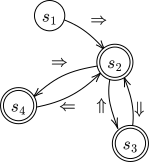
\includegraphics{../imgs/reverseengineering.pdf}
        \caption{Abstract state diagram (1).}
    \end{figure}
\end{problem}

\subsection*{Finite and Infinite Automata}

\begin{problem}
    [Unravelling a Language]
    Draw a state diagram of all of the languages that are reachable from the language \(L = \{\varepsilon, aa, ba, cab, c, acab\}\) in the Brzozowski automaton (by taking derivatives). 
    Include all of the double-circles to indicate which languages are accepting states of the Brzozowski automaton.
    What language is accepted by \(L\)?
\end{problem}

\begin{problem}
    [Language Accepts Itself]
    Let \(L \subseteq A^*\) be any language. 
    Prove that \(\mathcal L(\mathcal A_{Brz}, L) \subseteq L\).
\end{problem}

\subsection*{Finitely Recognizable Languages}

\begin{problem}
    [Languages as Trees]
    Let \(A = \{0, 1\}\), and let \(L \subseteq A^*\) be a language from \(A\). 
    Prove that if \(L\) is finite, i.e., \(L = \{w_1, \dots, w_n\}\) for some \(n \in \mathbb N\), then \(L\) is finitely recognizable.
\end{problem}

\begin{problem}
    [Total vs Partial]
    Prove that \(\mathsf{DFin} = \mathsf{TDFin}\) by describing how to turn a deterministic automaton into a total deterministic automaton without changing the languages accepted by the states.
\end{problem}

\end{document}